\documentclass[12pt]{article}

%\usepackage[version=3]{mhchem} % Package for chemical equation typesetting
\usepackage{siunitx} % Provides the \SI{}{} and \si{} command for typesetting SI units
\usepackage{graphicx} % Required for the inclusion of images
\usepackage{natbib} % Required to change bibliography style to APA
\usepackage{amsmath} % Required for some math elements 
\usepackage{float}
\usepackage{amssymb}
\usepackage{enumitem}
%pakiety wspomagaj?ce i poprawiaj?ce sk?adanie tabel
\usepackage{supertabular}
\usepackage{array}
\usepackage{tabularx}
\usepackage{hhline}
\usepackage{graphicx} 
\usepackage{wrapfig}


\setlength\parindent{0pt} % Removes all indentation from paragraphs

\renewcommand{\labelenumi}{\alph{enumi}.} % Make numbering in the enumerate environment by letter rather than number (e.g. section 6)

\title{Newton's method} % Title

\author{Dominik \textsc{Koszkul} \\ Micha\l\ \textsc{Oleszczyk}} % Author name

\usepackage{geometry}

\newgeometry{tmargin=2cm, bmargin=2cm, lmargin=2cm, rmargin=2cm}

\begin{document}

\maketitle % Insert the title, author and date

\section{Introduce}
\subsection{Formulating optimization problem}
Problem, which needs to be solved, is to find minimum point in set non-linear, multidimensional function. If function has more than one minimum, algorithm is looking for the nearest local minimum from initial point. In this project method to find these special points is Newton's method. This algorithm allows to find local minimum points, but this particular method can be optimized by using other algorithm to find optimal step, which is used in the main optimization program. Thanks to this, whole algorithm can find the solution in a faster way.
\subsection{Newton's method}
Newton's method is a local optimization type algorithm. To implement the method, stop criteria should be also known. In this case we have three main stop criteria for Newton's method and one additional that ensures that program stops counting after exceeding maximum compute time.
\begin{enumerate}
\item $ <grad f(x) \cdot grad f(x)> \leqslant \epsilon_1 $
\item $ ||x_i-x_{i-1}|| \leqslant \epsilon_2 $
\item $ |f(x_i)-f(x_{i-1})| \leqslant \epsilon_3 $
\item max number of iterations
\end{enumerate}  
If one from these four criteria 

\vspace{3cm}

Newton's method in optimization is a numeric method, which is used to find local extrema in a defined, differentiable function \textit{f}. In this method we need to construct a sequence $x_n$ from initial point $x_0$ to $x_*$ such that $f'(x_*)=0$. Last point is a local extremum point which we  are looking for.
\subsubsection{The Newton's method iteration}
Let $x_0$ be a point 


\section{Examples}
\subsection{Function with four local minima}
Function equation:
\begin{equation}
y=x_1^4+x_2^4-0.62x_1^2-0.62x_2^2
\end{equation}

Function figures:
	\begin{figure}[H]
		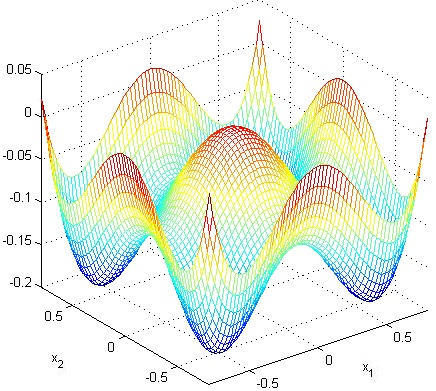
\includegraphics[width=12cm]{four_3d.jpg}
		\caption{Analyzed function 3D view.}
	\end{figure}
	\begin{figure}[H]
			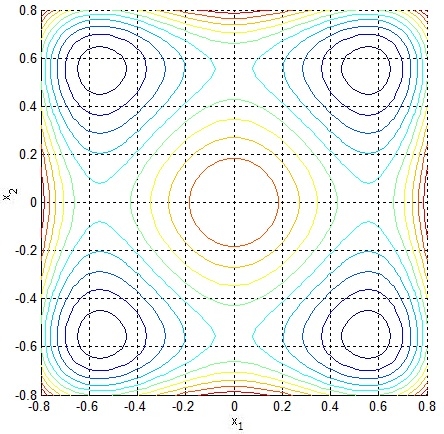
\includegraphics[width=12cm]{four_cont.jpg}
		\caption{Analyzed function contour view.}
	\end{figure}	

	\begin{table}[H]
		Results: \\ \\
		\begin{tabularx}{\textwidth}{c|X|c|c|c|c|}
			iteration & point coordinates & function value & $C_1$ value & $C_2$ value & $C_3$ value\\
			\hline
			0 & $1, 1$ & $0.76$ & $0.132$ & - & - \\
			\hline					
			1 & $0.743, 0.743$ & $-0.0743$ & $0.132$ & $0.363$ & $0.834$ \\ 
			\hline 
			2 & $0.61, 0.61$ & $-0.185$ & $0.0358$ & $0.189$ & $0.11$ \\ 
			\hline
			3 & $5.63\cdot10^{-1}, 5.63\cdot10^{-1}$  & $-1.92\cdot10^{-1}$ & $4.36\cdot10^{-3}$ & $6.6\cdot10^{-2}$ & $7.5\cdot10^{-3}$ \\ 
			\hline
			4 & $5.63\cdot10^{-1}, 5.63\cdot10^{-1}$  & $-1.92\cdot10^{-1}$ &
			$7.35\cdot10^{-5}$ & $6.6\cdot10^{-2}$ & $7.5\cdot10^{-3}$ \\ \hline
		\end{tabularx}	
	\end{table}		
	\begin{table}[H]
		\begin{tabularx}{\textwidth}{c|X|c|c|c|c|}
			iteration & point coordinates & function value & $C_1$ value & $C_2$ value & $C_3$ value\\
			\hline	
			0 & $-1, 1$ & $0.76$ & $0.132$ & - & - \\
			\hline					
			1 & $-0.743, 0.743$ & $-0.0743$ & $0.132$ & $0.363$ & $0.834$ \\ 
			\hline 
			2 & $-0.61, 0.61$ & $-0.185$ & $0.0358$ & $0.189$ & $0.11$ \\ 
			\hline
			3 & $-5.63\cdot10^{-1}, 5.63\cdot10^{-1}$  & $-1.92\cdot10^{-1}$ & $4.36\cdot10^{-3}$ & $6.6\cdot10^{-2}$ & $7.5\cdot10^{-3}$ \\ 
			\hline
			4 & $-5.63\cdot10^{-1}, 5.63\cdot10^{-1}$  & $-1.92\cdot10^{-1}$ &
			$7.35\cdot10^{-5}$ & $6.6\cdot10^{-2}$ & $7.5\cdot10^{-3}$ \\ \hline
		\end{tabularx}		 
	\end{table}
	\begin{table}[H]
		\begin{tabularx}{\textwidth}{c|X|c|c|c|c|}
			iteration & point coordinates & function value & $C_1$ value & $C_2$ value & $C_3$ value\\
			\hline	
			0 & $-1, -1$ & $0.76$ & $0.132$ & - & - \\
			\hline					
			1 & $-0.743, -0.743$ & $-0.0743$ & $0.132$ & $0.363$ & $0.834$ \\ 
			\hline 
			2 & $-0.61, -0.61$ & $-0.185$ & $0.0358$ & $0.189$ & $0.11$ \\ 
			\hline
			3 & $-5.63\cdot10^{-1}, -5.63\cdot10^{-1}$  & $-1.92\cdot10^{-1}$ & $4.36\cdot10^{-3}$ & $6.6\cdot10^{-2}$ & $7.5\cdot10^{-3}$ \\ 
			\hline
			4 & $-5.63\cdot10^{-1}, -5.63\cdot10^{-1}$  & $-1.92\cdot10^{-1}$ &
			$7.35\cdot10^{-5}$ & $6.6\cdot10^{-2}$ & $7.5\cdot10^{-3}$ \\ \hline
		\end{tabularx}		 
	\end{table}
	\begin{table}[H]
		\begin{tabularx}{\textwidth}{c|X|c|c|c|c|}
			iteration & point coordinates & function value & $C_1$ value & $C_2$ value & $C_3$ value\\
			\hline	
			0 & $1, -1$ & $0.76$ & $0.132$ & - & - \\
			\hline					
			1 & $0.743, -0.743$ & $-0.0743$ & $0.132$ & $0.363$ & $0.834$ \\ 
			\hline 
			2 & $0.61, -0.61$ & $-0.185$ & $0.0358$ & $0.189$ & $0.11$ \\ 
			\hline
			3 & $5.63\cdot10^{-1}, -5.63\cdot10^{-1}$  & $-1.92\cdot10^{-1}$ & $4.36\cdot10^{-3}$ & $6.6\cdot10^{-2}$ & $7.5\cdot10^{-3}$ \\ 
			\hline
			4 & $5.63\cdot10^{-1}, -5.63\cdot10^{-1}$  & $-1.92\cdot10^{-1}$ &
			$7.35\cdot10^{-5}$ & $6.6\cdot10^{-2}$ & $7.5\cdot10^{-3}$ \\ \hline
		\end{tabularx}		 
	\end{table}
	
	\begin{figure}[H]
		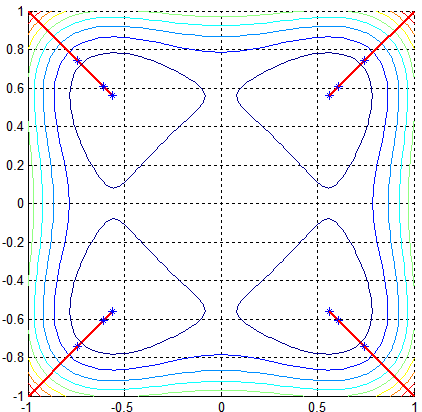
\includegraphics[width=16cm]{four_results.png}
		\caption{Location of four minima.}
	\end{figure}
	
\end{document}